\scanpage{72}
découpage pantalonique d'une carte (triangulée)

\figure{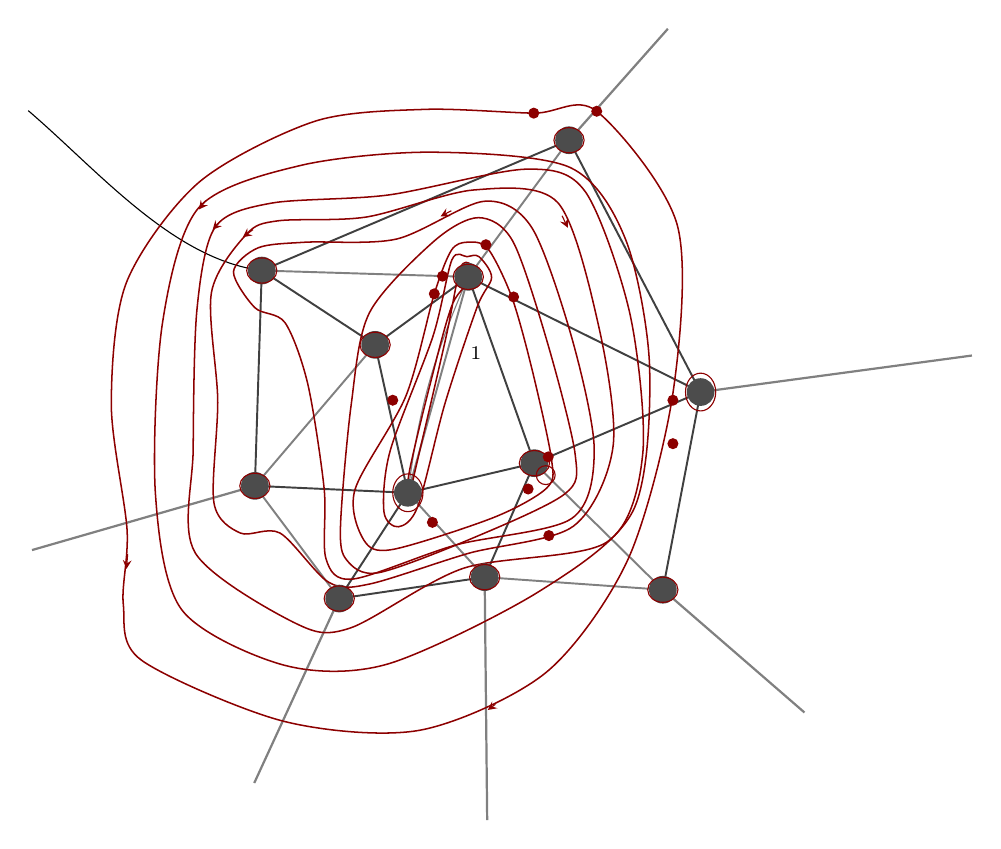
\begin{tikzpicture}[x=.008cm,y=-.008cm,>=stealth]
\coordinate (a) at (585,470);
\coordinate (b) at (1073,263);
\coordinate (c) at (913,480);
\coordinate (d) at (765,588);
\coordinate (e) at (574,812);
\coordinate (f) at (817,823);
\coordinate (g) at (1018,776);
\coordinate (h) at (1282,663);
\coordinate (i) at (708,991);
\coordinate (j) at (939,957);
\coordinate (k) at (1222,977);
\draw[black!75,line width=.7pt] (a)--(b);
\draw[gray,line width=.7pt] (a)--(c);
\draw[black!75,line width=.7pt] (a)--(d);
\draw[black!75,line width=.7pt] (a)--(e);
\draw[gray,line width=.7pt] (b)--(c);
\draw[black!75,line width=.7pt] (b)--(h);
\draw[black!75,line width=.7pt] (c)--(d);
\draw[gray,line width=.7pt] (c)--(f);
\draw[black!75,line width=.7pt] (c)--(g);
\draw[black!75,line width=.7pt] (c)--(h);
\draw[gray,line width=.7pt] (d)--(e);
\draw[black!75,line width=.7pt] (d)--(f);
\draw[black!75,line width=.7pt] (e)--(f);
\draw[gray,line width=.7pt] (e)--(i);
\draw[black!75,line width=.7pt] (f)--(g);
\draw[black!75,line width=.7pt] (f)--(i);
\draw[gray,line width=.7pt] (f)--(j);
\draw[black!75,line width=.7pt] (g)--(h);
\draw[black!75,line width=.7pt] (g)--(j);
\draw[gray,line width=.7pt] (g)--(k);
\draw[black!75,line width=.7pt] (h)--(k);
\draw[black!75,line width=.7pt] (i)--(j);
\draw[gray,line width=.7pt] (j)--(k);
\draw[gray] (c) to[bend right=8] (f);
\draw[gray,line width=.8pt] (b)--(1230,86);
\draw[gray,line width=.8pt] (e)--(220,914);
\draw[gray,line width=.8pt] (i)--(573,1284);
\draw[gray,line width=.8pt] (j)--(943,1343);
\draw[gray,line width=.8pt] (k)--(1447,1172);
\draw[gray,line width=.8pt] (h)--(1713,605);
\draw[black] (a) .. controls (443,452) and (324,310) .. (214,216);
\draw[red!55!black,line width=.55pt] plot[smooth cycle,tension=.5] coordinates {(1117,217) (1245,398) (1238,665) (1167,928) (1037,1108) (837,1200) (620,1186) (394,1089) (365,1000) (371,882) (346,684) (370,489) (485,330) (669,233) (844,214) (1017,220)};
\draw[red!55!black,line width=.55pt] plot[smooth cycle,tension=.5] coordinates {(485,370) (427,555) (416,824) (458,1009) (621,1097) (785,1095) (1025,980) (1175,851) (1201,624) (1163,421) (1074,306) (854,282) (647,303)};
\draw[red!55!black,line width=.55pt] plot[smooth cycle,tension=.5] coordinates {(511,401) (482,532) (476,754) (479,918) (638,1030) (725,1038) (905,943) (1132,902) (1190,762) (1170,540) (1099,345) (1005,309) (786,350) (600,363)};
\draw[red!55!black,line width=.55pt] plot[smooth cycle,tension=.5] coordinates {(561,412) (505,505) (515,676) (509,839) (551,887) (614,887) (691,965) (756,968) (914,919) (1080,876) (1143,749) (1120,558) (1055,362) (922,342) (751,385) (611,391)};
\draw[red!55!black,line width=.55pt] plot[smooth cycle,tension=.5] coordinates {(579,434) (540,472) (574,529) (622,553) (658,650) (684,816) (687,928) (730,960) (893,906) (1077,864) (1113,755) (1078,579) (1014,402) (938,360) (799,420) (654,425)};
\draw[red!55!black,line width=.55pt] plot[smooth cycle,tension=.5] coordinates {(756,537) (727,683) (710,876) (720,930) (770,950) (920,895) (1066,825) (1083,764) (1040,589) (984,424) (929,386) (859,423)};
\draw[red!55!black,line width=.55pt] plot[smooth cycle,tension=.5] coordinates {(859,507) (814,669) (733,818) (747,898) (793,913) (954,862) (1038,815) (1045,769) (1014,626) (982,512) (944,435) (911,425) (886,438)};
\draw[red!55!black,line width=.55pt] plot[smooth cycle,tension=.5] coordinates {(887,453) (857,574) (789,756) (779,853) (802,877) (833,844) (876,681) (927,528) (950,481) (930,448) (911,448)};
\draw[red!55!black,line width=.55pt] plot[smooth cycle,tension=.5] coordinates {(900,467) (878,574) (835,760) (816,838) (820,786) (853,648) (888,523) (923,479) (917,460)};
\fill[black!70] (a) circle (5pt);
\draw[red!55!black] (a) ellipse (24 and 20);
\fill[black!70] (b) circle (5pt);
\draw[red!55!black] (b) ellipse (24 and 20);
\fill[black!70] (c) circle (5pt);
\draw[red!55!black] (c) ellipse (24 and 20);
\fill[black!70] (d) circle (5pt);
\draw[red!55!black] (d) ellipse (24 and 20);
\fill[black!70] (e) circle (5pt);
\draw[red!55!black] (e) ellipse (24 and 20);
\fill[black!70] (f) circle (5pt);
\draw[red!55!black] (f) ellipse (24 and 30);
\fill[black!70] (g) circle (5pt);
\draw[red!55!black] (g) ellipse (24 and 20);
\fill[black!70] (h) circle (5pt);
\draw[red!55!black] (h) ellipse (24 and 30);
\fill[black!70] (i) circle (5pt);
\draw[red!55!black] (i) ellipse (24 and 20);
\fill[black!70] (j) circle (5pt);
\draw[red!55!black] (j) ellipse (24 and 20);
\fill[black!70] (k) circle (5pt);
\draw[red!55!black] (k) ellipse (24 and 20);
\draw[red!55!black] (1036,795) circle (15);
\fill[red!55!black] (1117,217) circle (2pt);
\fill[red!55!black] (1017,220) circle (2pt);
\fill[red!55!black] (941,429) circle (2pt);
\fill[red!55!black] (872,479) circle (2pt);
\fill[red!55!black] (859,507) circle (2pt);
\fill[red!55!black] (985,512) circle (2pt);
\fill[red!55!black] (793,676) circle (2pt);
\fill[red!55!black] (1040,766) circle (2pt);
\fill[red!55!black] (1238,745) circle (2pt);
\fill[red!55!black] (1238,676) circle (2pt);
\fill[red!55!black] (856,870) circle (2pt);
\fill[red!55!black] (1008,817) circle (2pt);
\fill[red!55!black] (1041,891) circle (2pt);
\draw[->,red!55!black] (496,359)--(485,373);
\draw[->,red!55!black] (519,392)--(507,405);
\draw[->,red!55!black] (571,405)--(555,417);
\draw[->,red!55!black] (886,375)--(869,384);
\draw[->,red!55!black] (1062,383)--(1071,402);
\draw[->,red!55!black] (956,1159)--(944,1168);
\draw[->,red!55!black] (372,920)--(370,944);
\node[font=\scriptsize] at (925,601) {$\unsure{1}$};
\end{tikzpicture}}
% crop-candidate: scan 72


\figure{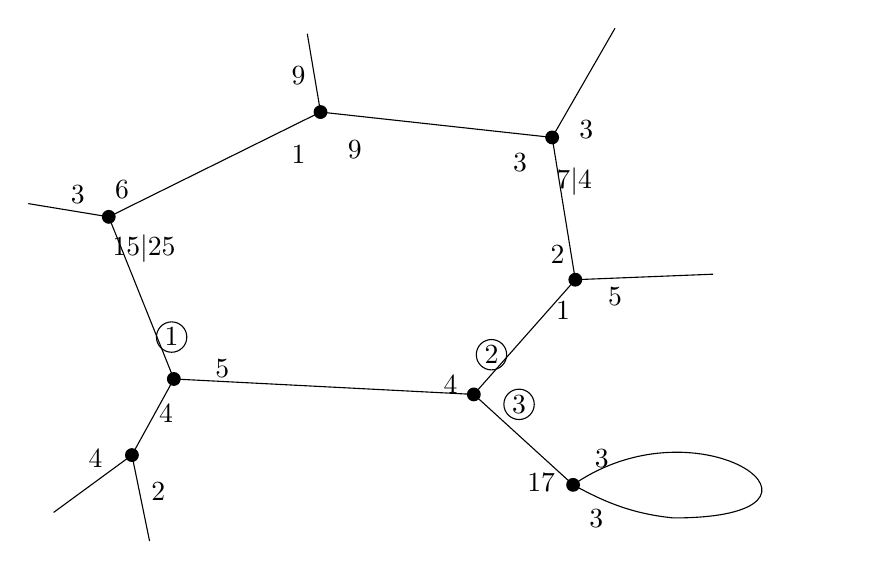
\begin{tikzpicture}[x=.014cm,y=-.014cm]
\coordinate (a) at (1558,821); \coordinate (b) at (1750,726);
\coordinate (c) at (1960,749); \coordinate (d) at (1981,878);
\coordinate (e) at (1889,982); \coordinate (f) at (1617,968);
\coordinate (g) at (1579,1037); \coordinate (h) at (1979,1064);
\draw (a)--(b)--(c)--(d)--(e)--(f)--cycle;
\draw (f)--(g) (e)--(h);
\draw (a)--(1485,809) (b)--(1738,655) (c)--(2017,650);
\draw (d)--(2106,873);
\draw (g)--(1508,1089) (g)--(1595,1115);
\draw (h) .. controls (2096,983) and (2245,1094) .. (2070,1094) .. controls (2030,1090) and (2005,1078) .. (h);
\foreach \p in {a,b,c,d,e,f,g,h} \fill (\p) circle (2.5pt);
\node at (1530,801) {$3$}; \node at (1570,796) {$6$};
\node at (1590,850) {$\unsure{15|25}$};
\node at (1730,693) {$9$}; \node at (1730,765) {$1$}; \node at (1781,760) {$9$};
\node at (1931,772) {$3$}; \node at (1991,742) {$3$}; \node at (1980,789) {$\unsure{7|4}$};
\node at (1965,855) {$2$}; \node at (1970,906) {$1$}; \node at (2017,893) {$5$};
\node at (1868,973) {$4$};
\node[draw,circle,inner sep=1pt] at (1905,946) {$2$};
\node[draw,circle,inner sep=1pt] at (1930,991) {$3$};
\node[draw,circle,inner sep=1pt] at (1615,930) {$1$};
\node at (1661,959) {$5$}; \node at (1610,999) {$4$};
\node at (1546,1040) {$4$}; \node at (1603,1070) {$2$};
\node at (1950,1062) {$17$}; \node at (2005,1040) {$3$}; \node at (2000,1095) {$3$};
\end{tikzpicture}}

\mspage{71}
